%%This is a very basic article template.
%%There is just one section and two subsections.
\documentclass{article}
\usepackage[francais]{babel}
\usepackage[T1]{fontenc}
\usepackage[latin1]{inputenc}
\usepackage[left=1cm, right=1cm, top=6mm, bottom=6mm]{geometry}
\usepackage{float}
\usepackage{graphicx}
\usepackage{array}
\usepackage{multirow}
\usepackage{amsmath, amssymb, mathrsfs}

\begin{document}
\begin{flushleft}
NOM PRENOM: \ldots \ldots \ldots \ldots \ldots \ldots \ldots \ldots \ldots

\bigskip
\end{flushleft}
\begin{center}
{\fbox{$2^{de}5$ \qquad \qquad \textbf{\Large{Contr�le de cours 2  (sujet 1)}}
\qquad \qquad 27/11/2008}}
\end{center}

\bigskip
\bigskip
Completer le tableau ci-dessous : 

\bigskip
\begin{tabular}{|m{55mm}|c|m{20mm}|m{20mm}|m{35mm}|}
\hline
Phrase contenant le mot distance & Encadrement & Valeur \qquad absolue & Intervalle  & Repr�sentation sur une droite
gradu�e\\
\hline
&$-5\leqslant x \leqslant 5$ & & & \\[7mm]
\hline
La distance de $x$ � $3$ est $6$& & & & \\[7mm]
\hline
& & & $x\in [-4;2]$& \\[7mm]
\hline
& & $|x-1|\leqslant2$& & \\[7mm]
\hline
& & & &\enskip  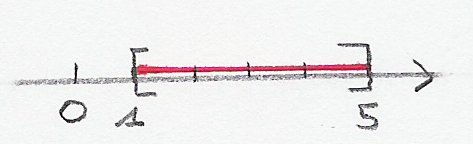
\includegraphics[width=35mm]{images/15.jpg} \\[7mm]
\hline
\end{tabular}

\bigskip
\bigskip
\bigskip
\bigskip

\begin{flushleft}
NOM PRENOM: \ldots \ldots \ldots \ldots \ldots \ldots \ldots \ldots \ldots

\bigskip
\end{flushleft}
\begin{center}
{\fbox{$2^{de}5$ \qquad \qquad \textbf{\Large{Contr�le de cours 2  (sujet 2)}}
\qquad \qquad 27/11/2008}}
\end{center}

\bigskip
\bigskip
Completer le tableau ci-dessous : 

\bigskip
\begin{tabular}{|m{55mm}|c|m{20mm}|m{20mm}|m{35mm}|}
\hline
Phrase contenant le mot distance & Encadrement & Valeur \qquad absolue & Intervalle  & Repr�sentation sur une droite
gradu�e\\
\hline
&$-4\leqslant x \leqslant 4$ & & & \\[7mm]
\hline
La distance de $x$ � $1$ est $4$& & & & \\[7mm]
\hline
& & & $x\in [-2;4]$& \\[7mm]
\hline
& & $|x-2|\leqslant 3$& & \\[7mm]
\hline
& & & &\enskip 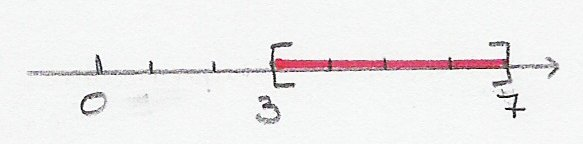
\includegraphics[width=35mm]{images/37.jpg} \\[7mm]
\hline
\end{tabular}

\end{document}
